
\subsection{Implement\'aci\'o}

\subsubsection{Architekt\'ura}
Az alkalmaz\'as k\'etr\'eteg\H u modell-n\'ezet architekt\'ura szerint k\'esz\"ult.
Ezek m\H uk\"od\'es\'et a \code{VisaulizationApplication} oszt\'aly k\"oti \"ossze \'es ir\'any\'itja.

\paragraph{Alkalmaz\'as}
\begin{figure}[h]
	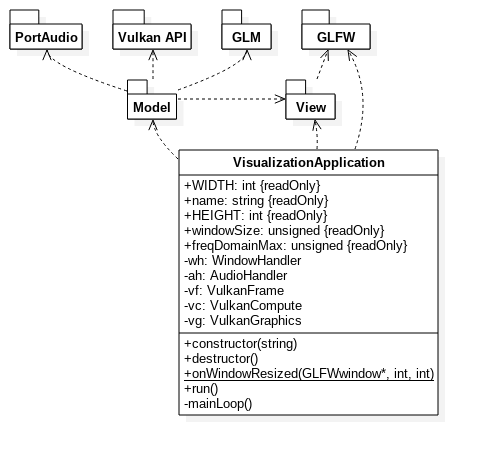
\includegraphics[width=\textwidth]{VisualizationApplication__VisualizationApp_0}
	\centering
	\caption{Az alkalmaz\'as oszt\'alydiagramja \'es a csomagkapcsolatok}
\end{figure}

Az alkalmaz\'as nev\'et a konstruktorban lehet be\'all\'itani, majd a \code{run} met\'odussal elind\'itani. \'Igy a \code{src/main.cpp} f\'ajlban tal\'alhat\'o \code{main} f\"uggv\'enynek csak az alkalmaz\'as futtat\'asa \'es a program sor\'an eldobott kiv\'etelek legv\'egs\H o elkap\'asa lesz a feladata.
Maga az alkalmaz\'as a k\"ovetkez\H o v\'altoz\'okon kereszt\"ul param\'eterezhet\H o:
\begin{itemize}
	\item \code{WIDTH} \'es \code{HEIGHT}: a megjelen\'it\H o ablak kezdeti m\'erete.
	\item \code{windowSize}: mekkora legyen a minta, amit elemz\"unk; a specifik\'aci\'oban $N$
\end{itemize}

\paragraph{N\'ezet}
\begin{figure}[h]
	\includegraphics[width=\textwidth]{View__ViewClassDiagram_2}
	\centering
	\caption{A n\'ezet r\'eteg}
\end{figure}
Az alkalmaz\'as fel\"ulete egy darab megjelen\'it\H o ablakb\'ol \'all, ez a prezent\'aci\'os fel\"ulet.
Ezt a \code{WindowHandler} oszt\'aly biztos\'itja, a GLFW k\"onyvt\'ar seg\'its\'eg\'evel. \newline
A konstruktor\'aban inicializ\'alja a GLFW-t, l\'etrehozza \'es be\'all\'itja az ablakot, be\'all\'itja a hibakezel\H o f\"uggv\'eny\'et. \newline
A \code{getGLFWextensions} f\"uggv\'ennyel inform\'aci\'ot szerezhet\"unk a k\"onyvt\'art\'ol, hogy milyen kieg\'esz\'it\H o funkcionalit\'asokra lesz sz\"uks\'eg\"unk a z\"okken\H omentes m\H uk\"od\'eshez. Ezt felhaszn\'aljuk amikor egy kompatibilis fizikai eszk\"ozt keres\"unk.

\paragraph{Modell}
A modell r\'eteg tov\'abbi r\'eszekre bonthat\'o.
\begin{figure}[h]
	\includegraphics{}
\end{figure}

\subparagraph{Hangkezel\'es}
A hang kezel\'es\'et az \code{AudioHandler} oszt\'aly biztos\'itja.
TODO: interf\'essz\'e alak\'it\'as, \'es k\"ul\"on TestAudioHandler illetve MicAudioHandler.

\subparagraph{Hangfeldolgoz\'as}
A hangfeldolgoz\'as a specifik\'aci\'oban eml\'itett m\'odon diszkr\'et Fourier-transzform\'aci\'oval t\"ort\'enik, ami a \code{VulkanCompute} oszt\'aly seg\'its\'eg\'evel vide\'ok\'arty\'an t\"ort\'enik.
A konstruktor\'aban l\'etrehozza a m\H uk\"od\'es\'ehez sz\"uks\'eges eszk\"oz\"oket. 
\begin{itemize}
	\item A logikai eszk\"ozt, amin kereszt\"ul a program a fizikai eszk\"ozzel kommunik\'alni tud.
	\item A logikai eszk\"ozh\"oz tartoz\'o sort, ahova az utas\'it\'asokat lehet k\"uldeni.
	\item Mem\'ori\'at allok\'al az eszk\"ozon.
	\item Buffereket hoz l\'etre a mem\'oria el\'er\'es\'ere.
	\item L\'etrehozza az er\H oforr\'as le\'ir\'okat.
	\item Bet\"olti a sz\'am\'it\'ast defini\'al\'o shadert.
	\item Sz\'am\'it\'asi cs\H ovezet\'eket hoz l\'etre.
	\item Command pool-t kre\'al \'es command buffer-t foglal bel\H ole.
	\item Felveszi a majd v\'egrehajtand\'o parancsokat a command buffer-be.
\end{itemize}

Ezek ut\'an haszn\'alatra k\'esz, amely sorrendje:
\begin{enumerate}
	\item Adatok felt\"olt\'ese a mem\'ori\'aba a \code{copyDataToGPU} f\"uggv\'eny seg\'its\'eg\'evel.
	\item A sz\'am\'it\'as futtat\'asa a \code{runCommandBuffer} met\'odus megh\'iv\'asa \'altal.
	\item A sz\'amolt eredm\'eny kiolvas\'as\'a a \code{readDataFromGPU} f\"uggv\'ennyel.
\end{enumerate}
TODO: A sz\'amol\'o \'es a rajzol\'o haszn\'aljon k\"oz\"os mem\'ori\'at.

\subparagraph{Rajzol\'as}
